% !Mode:: "TeX:UTF-8"
% !TEX program = xelatex

%%%%%%%%%% Port for macOS %%%%%%%%%%%
% Modified: Qin Yubo

\def\usewhat{xelatex}
\documentclass[12pt,openany,oneside]{ctexbook}
% 本科生毕业论文通常采用单页排版
% !Mode:: "TeX:UTF-8"
%  Authors: 张井   Jing Zhang: prayever@gmail.com     天津大学2010级管理与经济学部信息管理与信息系统专业硕士生
%           余蓝涛 Lantao Yu: lantaoyu1991@gmail.com  天津大学2008级精密仪器与光电子工程学院测控技术与仪器专业本科生

%%%%%%%%%% Package %%%%%%%%%%%%
\usepackage{CJK}
\usepackage{setspace}
\usepackage{etoolbox}                       % patch: 进行hack
\usepackage{lmodern}
\usepackage[T1]{fontenc}
\usepackage{graphicx}                       % 支持插图处理
% \usepackage[a4paper,text={146.4true mm,239.2 true mm},top= 26.2true mm,left=31.8 true mm,head=6true mm,headsep=6.5true mm,foot=16.5true mm]{geometry}
%
% 设置页面边距
\usepackage[a4paper,
top=27.5true mm, % 顶部边距
bottom=25.4true mm, % 底部边距
left=35.7true mm, % 左侧边距
right=27.7true mm, % 右侧边距
headheight=15true mm, % 页眉高度
% headsep=15true mm, % 页眉距顶部边界的距离
headsep=5true mm, % 页眉距顶部边界的距离
footskip=17.5true mm % 页脚距底部边界的距离
]{geometry}
% 支持版面尺寸设置
\usepackage[squaren]{SIunits}               % 支持国际标准单位
\usepackage{titlesec}                       % 控制标题的宏包
\usepackage{titletoc}                       % 控制目录的宏包
\usepackage{fancyhdr}                       % fancyhdr宏包 支持页眉和页脚的相关定义
%\usepackage{ctex}                     % 支持中文显示
\usepackage{CJKpunct}                       % 精细调整中文的标点符号
\usepackage{color}                          % 支持彩色
\usepackage{mathtools}
\usepackage{amsmath}                        % AMSLaTeX宏包 用来排出更加漂亮的公式
\usepackage{amssymb}                        % 数学符号生成命令
\usepackage[below]{placeins}    %允许上一个section的浮动图形出现在下一个section的开始部分,还提供\FloatBarrier命令,使所有未处理的浮动图形立即被处理
\usepackage{multirow}                       % 使用Multirow宏包,使得表格可以合并多个row格
\usepackage{booktabs}                       % 表格,横的粗线;\specialrule{1pt}{0pt}{0pt}
\usepackage{longtable}                      % 支持跨页的表格。
\usepackage{tabularx}                       % 自动设置表格的列宽
% \usepackage{subfigure}                      % 支持子图 %centerlast 设置最后一行是否居中
\usepackage{ccaption}            % 支持子图的中文标题
% \usepackage{subfig}
\usepackage{subcaption}                     % 用于子图和子标题 (subfigure和subfig已经obsolete)
\usepackage[sort&compress,numbers]{natbib}  % 支持引用缩写的宏包
\usepackage{enumitem}                       % 使用enumitem宏包,改变列表项的格式
\usepackage{calc}                           % 长度可以用+ - * / 进行计算
\usepackage{newtxtext}                      % 用newtxtext宏包替代txfonts
% \usepackage{txfonts}                        % 字体宏包
\usepackage{bm}                             % 处理数学公式中的黑斜体的宏包
\usepackage[amsmath,thmmarks,hyperref]{ntheorem}  % xxx 定理类环境宏包,其中 amsmath 选项用来兼容 AMS LaTeX 的宏包
\usepackage{CJKnumb}                        % 提供将阿拉伯数字转换成中文数字的命令
\usepackage{indentfirst}                    % 首行缩进宏包
\usepackage{CJKutf8}                        % 用在UTF8编码环境下,它可以自动调用CJK,同时针对UTF8编码作了设置
\usepackage{xeCJK}
%\usepackage{hypbmsec}                      % 用来控制书签中标题显示内容
\newcommand{\tabincell}[2]{\begin{tabulngar}{@{}#1@{}}#2\end{tabular}}
\usepackage{xcolor}
%支持代码环境
\usepackage{listings}
\lstset{numbers=left,
  language=[ANSI]{C},
  numberstyle=\tiny,
  extendedchars=false,
  showstringspaces=false,
  breakatwhitespace=false,
  breaklines=true,
  captionpos=b,
  keywordstyle=\color{blue!70},
  commentstyle=\color{red!50!green!50!blue!50},
  frame=shadowbox,
  rulesepcolor=\color{red!20!green!20!blue!20}
}
%支持算法环境
% \usepackage[boxed,ruled,lined]{algorithm2e}
% \usepackage{algorithmic}
\usepackage{algorithm}
\usepackage{algorithmicx}  % 更好的算法包
\usepackage{algpseudocode}

\usepackage{array}
\renewcommand{\arraystretch}{1.5} % 调整行间距为默认的1.5倍

\usepackage{pdfpages}

\newcommand{\PreserveBackslash}[1]{\let\temp=\\#1\let\\=\temp}
\newcolumntype{C}[1]{>{\PreserveBackslash\centering}p{#1}}
\newcolumntype{R}[1]{>{\PreserveBackslash\raggedleft}p{#1}}
\newcolumntype{L}[1]{>{\PreserveBackslash\raggedright}p{#1}}

\def\atemp{xelatex}\ifx\atemp\usewhat
  \usepackage[unicode,
  pdfstartview=FitH,
  bookmarksnumbered=true,
  bookmarksopen=true,
  colorlinks=true, %false,
  pdfborder={0 0 1},
  citecolor=black, %blue,
  linkcolor=black, %red,
  anchorcolor=green,
  urlcolor=black, %blue,
  breaklinks=true
  ]{hyperref}
\fi
                                % 定义本文所使用宏包
\graphicspath{{figures/}}                            % 定义所有的图像文件在 figures 子目录下

\begin{document}                                     % 开始全文

% !Mode:: "TeX:UTF-8"
%  Authors: 张井   Jing Zhang: prayever@gmail.com     天津大学2010级管理与经济学部信息管理与信息系统专业硕士生
%           余蓝涛 Lantao Yu: lantaoyu1991@gmail.com  天津大学2008级精密仪器与光电子工程学院测控技术与仪器专业本科生

%%%%%%%%%%%%%%%%% Fonts Definition and Basics %%%%%%%%%%%%%%%%%
%\newcommand{\song}{\CJKfamily{song}}    % 宋体
%\newcommand{\fs}{\CJKfamily{fs}}        % 仿宋体
%\newcommand{\kai}{\CJKfamily{kai}}      % 楷体
%\newcommand{\hei}{\CJKfamily{hei}}      % 黑体
%\newcommand{\li}{\CJKfamily{li}}        % 隶书
\newcommand{\song}{\songti}    % 宋体
\newcommand{\fs}{\fangsong}        % 仿宋体
\newcommand{\kai}{\kaishu}      % 楷体
\newcommand{\hei}{\heiti}      % 黑体
\newcommand{\li}{\lishu}        % 隶书
\newcommand{\yihao}{\fontsize{26pt}{26pt}\selectfont}       % 一号, 单倍行距
\newcommand{\xiaoyi}{\fontsize{24pt}{24pt}\selectfont}      % 小一, 单倍行距
\newcommand{\erhao}{\fontsize{22pt}{1.25\baselineskip}\selectfont}       % 二号, 1.25倍行距
\newcommand{\xiaoer}{\fontsize{18pt}{18pt}\selectfont}      % 小二, 单倍行距
\newcommand{\sanhao}{\fontsize{16pt}{16pt}\selectfont}      % 三号, 单倍行距
\newcommand{\xiaosan}{\fontsize{15pt}{15pt}\selectfont}     % 小三, 单倍行距
\newcommand{\sihao}{\fontsize{14pt}{14pt}\selectfont}       % 四号, 单倍行距
\newcommand{\xiaosi}{\fontsize{12pt}{12pt}\selectfont}      % 小四, 单倍行距
\newcommand{\wuhao}{\fontsize{10.5pt}{10.5pt}\selectfont}   % 五号, 单倍行距
\newcommand{\xiaowu}{\fontsize{9pt}{9pt}\selectfont}        % 小五, 单倍行距

%\CJKtilde  % 重新定义了波浪符~的意义
% JUST DON'T USE CJK
% 使用 ctexbook 之后已无必要
\newcommand\prechaptername{第}
\newcommand\postchaptername{章}

\punctstyle{hangmobanjiao}             % 调整中文字符的表示,行内占一个字符宽度,行尾占半个字符宽度

% 调整罗列环境的布局
\setitemize{leftmargin=3em,itemsep=0em,partopsep=0em,parsep=0em,topsep=-0em}
\setenumerate{leftmargin=3em,itemsep=0em,partopsep=0em,parsep=0em,topsep=0em}

% 避免宏包 hyperref 和 arydshln 不兼容带来的目录链接失效的问题。
\def\temp{\relax}
\let\temp\addcontentsline
\gdef\addcontentsline{\phantomsection\temp}

% 自定义项目列表标签及格式 \begin{publist} 列表项 \end{publist}
\newcounter{pubctr} %自定义新计数器
\newenvironment{publist}{%%%%%定义新环境
\begin{list}{[\arabic{pubctr}]} %%标签格式
    {
     \usecounter{pubctr}
     \setlength{\leftmargin}{2.5em}   % 左边界 \leftmargin =\itemindent + \labelwidth + \labelsep
     \setlength{\itemindent}{0em}     % 标号缩进量
     \setlength{\labelsep}{1em}       % 标号和列表项之间的距离,默认0.5em
     \setlength{\rightmargin}{0em}    % 右边界
     \setlength{\topsep}{0ex}         % 列表到上下文的垂直距离
     \setlength{\parsep}{0ex}         % 段落间距
     \setlength{\itemsep}{0ex}        % 标签间距
     \setlength{\listparindent}{0pt}  % 段落缩进量
    }}
{\end{list}}

\makeatletter
\renewcommand\normalsize{
  \@setfontsize\normalsize{12pt}{12pt} % 小四对应 12 pt
  \setlength\abovedisplayskip{4pt}
  \setlength\abovedisplayshortskip{4pt}
  \setlength\belowdisplayskip{\abovedisplayskip}
  \setlength\belowdisplayshortskip{\abovedisplayshortskip}
  \let\@listi\@listI}
\def\defaultfont{\renewcommand{\baselinestretch}{1.63}\normalsize\selectfont} % 设置行距

\renewcommand{\CJKglue}{\hskip -0.1 pt plus 0.08\baselineskip} % 控制字间距,使每行 34 个汉字
\makeatother

%%%%%%%%%%%%% Contents %%%%%%%%%%%%%%%%%
\renewcommand{\contentsname}{目\qquad 录}
\setcounter{tocdepth}{2} % 控制目录深度
% 使用 ctexbook 之后已无必要
%\titlecontents{chapter}[2em]{\vspace{.5\baselineskip}\xiaosan\song}
             %{\prechaptername\CJKnumber{\thecontentslabel}\postchaptername\qquad}{}
             %{\hspace{.5em}\titlerule*[10pt]{$\cdot$}\sihao\contentspage}
\titlecontents{chapter}[2em]{\vspace{.5\baselineskip}\xiaosan\song}
             {\thecontentslabel\qquad}{}
             {\hspace{.5em}\titlerule*[10pt]{$\cdot$}\sihao\contentspage}
\titlecontents{section}[3em]{\vspace{.25\baselineskip}\sihao\song}
             {\thecontentslabel\quad}{}
             {\hspace{.5em}\titlerule*[10pt]{$\cdot$}\sihao\contentspage}
\titlecontents{subsection}[4em]{\vspace{.25\baselineskip}\sihao\song}
             {\thecontentslabel\quad}{}
             {\hspace{.5em}\titlerule*[10pt]{$\cdot$}\sihao\contentspage}

%%%%%%%%%% Chapter and Section %%%%%%%%%%%%%
\setcounter{secnumdepth}{4}
\setlength{\parindent}{2em}
\renewcommand{\chaptername}{\prechaptername\CJKnumber{\thechapter}\postchaptername}
\titleformat{\chapter}{\centering\xiaosan\song}{\hei\chaptername}{2em}{}
\titlespacing{\chapter}{0pt}{0.1\baselineskip}{0.8\baselineskip}
\titleformat{\section}{\sihao\hei}{\thesection}{1em}{}
\titlespacing{\section}{0pt}{0.15\baselineskip}{0.25\baselineskip}
\titleformat{\subsection}{\sihao\hei}{\thesubsection}{1em}{}
\titlespacing{\subsection}{0pt}{0.1\baselineskip}{0.3\baselineskip}
\titleformat{\subsubsection}{\sihao\hei}{\thesubsubsection}{1em}{}
\titlespacing{\subsubsection}{0pt}{0.05\baselineskip}{0.1\baselineskip}

%%%%%%%%%% Table, Figure and Equation %%%%%%%%%%%%%%%%%
\renewcommand{\tablename}{表}                                     % 插表题头
\renewcommand{\figurename}{图}                                    % 插图题头
\renewcommand{\thefigure}{\arabic{chapter}-\arabic{figure}}       % 使图编号为 7-1 的格式 %\protect{~}
\renewcommand{\thesubfigure}{\alph{subfigure})}                   % 使子图编号为 a) 的格式
\renewcommand{\thesubtable}{(\alph{subtable})}                    % 使子表编号为 (a) 的格式
\renewcommand{\thetable}{\arabic{chapter}-\arabic{table}}         % 使表编号为 7-1 的格式
\renewcommand{\theequation}{\arabic{chapter}-\arabic{equation}}   % 使公式编号为 7-1 的格式
\newcommand{\ud}{\mathrm{d}}

%%%%%% 定制浮动图形和表格标题样式 %%%%%%
\makeatletter
\long\def\@makecaption#1#2{
   \vskip\abovecaptionskip
   \sbox\@tempboxa{\centering\wuhao\song{#1\qquad #2} }
   \ifdim \wd\@tempboxa >\hsize
     \centering\wuhao\song{#1\qquad #2} \par
   \else
     \global \@minipagefalse
     \hb@xt@\hsize{\hfil\box\@tempboxa\hfil}
   \fi
   \vskip\belowcaptionskip}
\makeatother
\captiondelim{~~~~} %用来控制longtable表头分隔符

%%%%%%%%%% Theorem Environment %%%%%%%%%%%%%%%%%
\theoremstyle{plain}
\theorembodyfont{\song\rmfamily}
\theoremheaderfont{\hei\rmfamily}
\newtheorem{theorem}{定理~}[chapter]
\newtheorem{lemma}{引理~}[chapter]
\newtheorem{axiom}{公理~}[chapter]
\newtheorem{proposition}{命题~}[chapter]
\newtheorem{prop}{性质~}[chapter]
\newtheorem{corollary}{推论~}[chapter]
\newtheorem{definition}{定义~}[chapter]
\newtheorem{conjecture}{猜想~}[chapter]
\newtheorem{example}{例~}[chapter]
\newtheorem{remark}{注~}[chapter]
%\newtheorem{algorithm}{算法~}[chapter]
\newenvironment{proof}{\noindent{\hei 证明:}}{\hfill $ \square $ \vskip 4mm}
\theoremsymbol{$\square$}

%%%%%%%%%% Page: number, header and footer  %%%%%%%%%%%%%%%%%

%\frontmatter 或 \pagenumbering{roman}
%\mainmatter 或 \pagenumbering{arabic}
\makeatletter
\renewcommand\frontmatter{\clearpage
  \@mainmatterfalse
  }
\makeatother

%%%%%%%%%%% Code: Listings from MCM Template %%%%%%%%%%%%

\definecolor{grey}{rgb}{0.8,0.8,0.8}
\definecolor{darkgreen}{rgb}{0,0.3,0}
\definecolor{darkblue}{rgb}{0,0,0.3}
\def\lstbasicfont{\fontfamily{pcr}\selectfont\footnotesize}
\lstset{%
% indexing
   % numbers=left,
   % numberstyle=\small,%
% character display
    showstringspaces=false,
    showspaces=false,%
    tabsize=4,%
% style
    frame=lines,%
    basicstyle={\footnotesize\lstbasicfont},%
    keywordstyle=\color{darkblue}\bfseries,%
    identifierstyle=,%
    commentstyle=\color{darkgreen},%\itshape,%
    stringstyle=\color{black}%
}
\lstloadlanguages{C,C++,Java,Matlab,Mathematica,Python}

%%%%%%%%%%%% References %%%%%%%%%%%%%%%%%
\renewcommand{\bibname}{参考文献}
% 重定义参考文献样式,来自thu
\makeatletter
\renewenvironment{thebibliography}[1]{
    \titleformat{\chapter}{\raggedright\sihao\hei}{\chaptername}{2em}{}
   \chapter*{\bibname}
   \wuhao
   \list{\@biblabel{\@arabic\c@enumiv}}
        {\renewcommand{\makelabel}[1]{##1\hfill}
         \settowidth\labelwidth{0 cm}
         \setlength{\labelsep}{0pt}
         \setlength{\itemindent}{0pt}
         \setlength{\leftmargin}{\labelwidth+\labelsep}
         \addtolength{\itemsep}{-0.7em}
         \usecounter{enumiv}
         \let\p@enumiv\@empty
         \renewcommand\theenumiv{\@arabic\c@enumiv}}
    \sloppy\frenchspacing
    \clubpenalty4000
    \@clubpenalty \clubpenalty
    \widowpenalty4000
    \interlinepenalty4000
    \sfcode`\.\@m}
   {\def\@noitemerr
     {\@latex@warning{Empty `thebibliography' environment}}
    \endlist\frenchspacing}
\makeatother

\addtolength{\bibsep}{-0.5em}     % 缩小参考文献间的垂直间距
\setlength{\bibhang}{2em}         % 每个条目自第二行起缩进的距离

% 参考文献引用作为上标出现
%\newcommand{\citeup}[1]{\textsuperscript{\cite{#1}}}
\makeatletter
    \def\@cite#1#2{\textsuperscript{[{#1\if@tempswa , #2\fi}]}}
\makeatother
%% 引用格式
\bibpunct{[}{]}{,}{s}{}{,}

%%%%%%%%%%%% Cover %%%%%%%%%%%%%%%%%
% 封面、摘要、版权、致谢格式定义
\makeatletter
\def\ctitle#1{\def\@ctitle{#1}}\def\@ctitle{}
\def\cdegree#1{\def\@cdegree{#1}}\def\@cdegree{}
\def\caffil#1{\def\@caffil{#1}}\def\@caffil{}
\def\csubject#1{\def\@csubject{#1}}\def\@csubject{}
\def\cgrade#1{\def\@cgrade{#1}}\def\@cgrade{}
\def\cauthor#1{\def\@cauthor{#1}}\def\@cauthor{}
\def\cnumber#1{\def\@cnumber{#1}}\def\@cnumber{}
\def\csupervisor#1{\def\@csupervisor{#1}}\def\@csupervisor{}
\def\crank#1{\def\@crank{#1}}\def\@crank{}
\def\cdate#1{\def\@cdate{#1}}\def\@cdate{}
\long\def\cabstract#1{\long\def\@cabstract{#1}}\long\def\@cabstract{}
\long\def\eabstract#1{\long\def\@eabstract{#1}}\long\def\@eabstract{}
\def\ckeywords#1{\def\@ckeywords{#1}}\def\@ckeywords{}
\def\ekeywords#1{\def\@ekeywords{#1}}\def\@ekeywords{}
\def\cheading#1{\def\@cheading{#1}}\def\@cheading{}


\pagestyle{fancy}
  \fancyhf{}
  \fancyhead[C]{\song\wuhao \@cheading}  % 页眉显示天津大学 20XX 届本科生毕业论文
  \fancyfoot[C]{\song\xiaowu ~\thepage~}
\newlength{\@title@width}

% 定义封面
\def\makecover{
%\cleardoublepage%
   \phantomsection
    \pdfbookmark[-1]{\@ctitle}{ctitle}

    \begin{titlepage}
      \vspace*{31.5pt}
      \begin{center}

  \begin{figure}[h]
  \centering
  
\includegraphics[width=0.4\textwidth]{figures/tjuname.eps}
  \end{figure}
  \vspace*{21pt}
  \hei\erhao{\textbf{本科生毕业论文}}
  \vspace*{52.5pt}

  \begin{figure}[h]
  \centering
  
\includegraphics[width=0.3\textwidth]{figures/tjulogo.eps}
  \end{figure}

  \vspace*{42pt}
  \renewcommand\arraystretch{1.5}
  \setlength{\@title@width}{5cm}
  {\sanhao\song{\bf{
  \begin{tabular}{lc}
    学\qquad 院&  \underline{\makebox[\@title@width][c]{\@caffil}} \\
    专\qquad 业 &  \underline{\makebox[\@title@width][c]{\@csubject}} \\
    年\qquad 级  &  \underline{\makebox[\@title@width][c]{\@cgrade}}\\
    姓\qquad 名 &  \underline{\makebox[\@title@width][c]{\@cauthor}} \\
    指导教师 &  \underline{\makebox[\@title@width][c]{\@csupervisor}} \\
  \end{tabular}}}
 }
  \vspace*{21pt}

\song\sanhao{\textbf{\@cdate}}
\end{center}
\end{titlepage}

%%%%%%%%%%%%%%%%%%%   Abstract and Keywords  %%%%%%%%%%%%%%%%%%%%%%%
\clearpage
\markboth{摘~要}{摘~要}
\pdfbookmark[0]{摘~~要}{cabstract}
%\addcontentsline{toc}{chapter}{摘~要}
%\chapter*{\centering\sanhao\hei\bfseries 摘\qquad 要}
\chapter*{\centering\sanhao\hei 摘\qquad 要}
\song\defaultfont
\@cabstract
\vspace{\baselineskip}

\hangafter=1\hangindent=52.3pt\noindent
{\hei\xiaosi 关键词:} \@ckeywords
\thispagestyle{empty}

%%%%%%%%%%%%%%%%%%%   English Abstract  %%%%%%%%%%%%%%%%%%%%%%%%%%%%%%
\clearpage
%\phantomsection
\markboth{ABSTRACT}{ABSTRACT}
\pdfbookmark[0]{ABSTRACT}{eabstract}
%\addcontentsline{toc}{chapter}{ABSTRACT}
\chapter*{\centering\sanhao{\bf{ABSTRACT}}}
%\vspace{\baselineskip}
\@eabstract
\vspace{\baselineskip}

\hangafter=1\hangindent=60pt\noindent
{\textbf{Keywords:}} \@ekeywords
\thispagestyle{empty}
}
\makeatother
                                 % 完成对论文各个部分格式的设置

\frontmatter                                         % 以下是论文导言部分,包括论文的封面,中英文摘要和中文目录
\fancypagestyle{plain}{
  \fancyhf{}
  \renewcommand{\headrulewidth}{0 pt}
  \fancyfoot[C]{\song\xiaowu~\thepage~}
}

% 直接从 Word 模板生成封面导出 pdf 似乎更方便
% !Mode:: "TeX:UTF-8"

%%  可通过增加或减少 setup/format.tex中的
%%  第274行 \setlength{\@title@width}{8cm}中 8cm 这个参数来 控制封面中下划线的长度。

\cheading{天津大学~2016~届本科生毕业论文}      % 设置正文的页眉,需要填上对应的毕业年份
\ctitle{基于顾客有限理性预期的定价与供应链结构}    % 封面用论文标题,自己可手动断行
\caffil{管理与经济学部} % 学院名称
\csubject{工业工程}   % 专业名称
\cgrade{2012~级}            % 年级
\cauthor{秦昱博}            % 学生姓名
\cnumber{3012209017}        % 学生学号
\csupervisor{杨道箭}        % 导师姓名
\crank{副教授}              % 导师职称

\cdate{\the\year~年~\the\month~月~\the\day~日}

\cdeclaration{
本人声明:所呈交的毕业设计(论文),是本人在指导教师指导下,进行研究工作所取得的成果。除文中已经注明引用的内容外,本毕业设计(论文)中不包含任何他人已经发表或撰写过的研究成果。对本毕业设计(论文)所涉及的研究工作做出贡献的其他个人和集体,均已在论文中作了明确的说明。本毕业设计(论文)原创性声明的法律责任由本人承担。
}

\cabstract{
中文摘要一般为300~400字,简要介绍毕业设计(论文)的研究目的、方法、结果和结论,语言力求精炼。英文摘要应与中文摘要相对应。中英文摘要均要有关键词,一般为3~8个,中英文摘要要相互对应。

中文摘要。“摘要”两字之间空一个全角空格或两个半角空格,字体为宋体二号字加粗,居中显示,摘要内容采用正文样式。中文关键词与摘要内容间隔一行,无缩进左对齐书写。“关键词:”采用宋体四号字加粗,关键词内容采用正文样式,且换行不缩进。关键词之间用逗号分隔。

英文摘要。此部分皆为Times New Roman字体。“ABSTRACT”为二号字加粗,居中显示。英文摘要内容采用正文样式。英文关键词与英文摘要内容间隔一行,无缩进左对齐书写。“KEY WORDS:”为四号字加粗,英文关键词采用正文样式,且换行不缩进,关键词之间用逗号分隔,词义和中文关键词相同。“ABSTRACT”和“KEY WORDS”一律用大写字母,每个关键词的首字母要大写。
}

\ckeywords{关键词~1;关键词~2;关键词~3;……;关键词~7(关键词总共~3~—~7~个,最后一个关键词后面没有标点符号)}

\eabstract{
The upper bound of the number of Chinese characters is 400. The abstract aims at introducing the research purpose, research methods, research results, and research conclusion of graduation thesis, with refining words. Generally speaking, both the Chinese and English abstracts require the keywords, the number of which varies from 3 to 7, with a semicolon between adjacent words. The font of the English Abstract is Times New Roman, with the size of 12pt(small four).
}

\ekeywords{keyword 1, keyword 2, keyword 3, ……, keyword 7 (no punctuation at the end)}

\makecover

\clearpage
                                % 封面

%%%%%%%%%%   目录   %%%%%%%%%%
\defaultfont
\clearpage{\pagestyle{empty}\cleardoublepage}

% \pagenumbering{arabic}

\titleformat{\chapter}{\centering\sanhaoup\hei}{\chaptername}{2em}{} % 设置目录两字的格式
\pdfbookmark[0]{目~~录}{mulu}
\tableofcontents                                     % 中文目录

% \fancypagestyle{plain}{
%   \fancyhf{}
%   \renewcommand{\headrulewidth}{0 pt}
%   \fancyfoot[C]{\song\xiaowu~\thepage~}
% }
% \thispagestyle{plain}

%%%%%%%%%%%%%%%%%%%%%%%%%%%%%%%%%%%%%%%%%%%%%%%%%%%%%%%%%%%


\mainmatter\defaultfont\sloppy\raggedbottom
\makeatletter
\fancypagestyle{plain}{                              % 设置开章页眉页脚风格
  \fancyhf{}
  \fancyhead[C]{\song\wuhao \@cheading}            % 首页页眉格式
  \fancyfoot[C]{\song\xiaowu ~\thepage~}           % 首页页脚格式
  \renewcommand{\headrulewidth}{0.5pt}
  \renewcommand{\footrulewidth}{0pt}
}

\setlength{\footskip}{15pt}

\makeatother
% \titleformat{\chapter}{\centering\xiaosan\hei}{\chaptername}{2em}{} % 恢复chapter标题格式要求

\iffalse
  \bibliography{reference/reference.bib} % 欺骗latextools获取bib文件
\fi

%%%%%%% 正文 %%%%%%%


\fontsize{12pt}{12pt}\selectfont

\setcounter{page}{1}                                 % 单独从 1 开始编页码
%%%%%%% Chapter 1 %%%%%%%


\chapter{绪论}

此处格式已按模板设定,作者只需选择段落区域,输入替换之。模版中所有说明性文字用于注释格式与内容的要求,撰写论文时请删除。模版中,图表、公式、参考文献等都已给出范例,撰写论文时请删除。

本模版已包含符合章节设置的“多级别列表”,只需在相应位置替换标题文字即可。如需增加章节,建议先使用格式刷,再调整编号。

\section{毕业设计(论文)类型及基本要求}

\subsection{设计类}

学生必须独立完成一定数量的设计图纸,撰写一篇15000字以上的设计说明书,工程设计类图纸折合成零号图纸不能少于三张。

\subsection{论文类}

学生必须独立完成一项研究或实验,撰写一篇15000字以上的论文。基础理论类的研究型论文的正文文字一般不少于10000字,要求内容充实,论据充分可靠,论证有力,主题明确。

\subsection{软件类}

学生必须独立完成一个软件或较大软件中的一个模块设计,撰写一篇15000字以上的设计说明书。

\section{毕业设计(论文)资料组成及存档要求}

毕业设计(论文)资料包括:任务书、开题报告、毕业设计(论文)、外文资料、中文译文、过程指导记录表、中期检查记录表、指导教师评阅书、评阅教师评阅书、答辩记录书,以及图纸、实验报告、计算程序等。

毕业设计(论文)的纸质版资料由各院、系自行安排保存,电子版资料在天津大学本科生毕业设计(论文)管理系统中保存,要保证两类资料的一致性。

毕业设计(论文)及图纸、实验报告、计算程序等装订成册(图纸数量过多可单独装订成册),附件资料按顺序装订成册(资料顺序为:附件封面、目录、任务书、开题报告、外文资料、中文译文、过程指导记录表、中期检查记录表、指导教师评阅书、评阅教师评阅书、答辩记录书),两册一并存档,两册封面均采用天津大学本科生毕业设计(论文)统一封面。

\chapter{理论研究}

此处格式已按模板设定,作者只需选择段落区域,输入替换之。模版中所有说明性文字用于注释格式与内容的要求,撰写论文时请删除。模版中,图表、公式、参考文献等都已给出范例,撰写论文时请删除。

本模版已包含符合章节设置的“多级别列表”,只需在相应位置替换标题文字即可。如需增加章节,建议先使用格式刷,再调整编号。

\section{毕业设计(论文)结构及要求}

\subsection{论文结构}

毕业设计(论文)原则上应采用中文完成(教学语言为英语的除外),确需用其他语言撰写的需经学院审批同意并报教务处备案。毕业设计(论文)一般由以下部分组成,依次为:①封面;②扉页;③独创性声明;④中英文摘要及关键词;⑤目录;⑥正文;⑦参考文献;⑧附录;⑨致谢。

\subsection{语言表述}

要做到数据可靠、推理严谨、立论正确。论述必须简明扼要、重点突出,对同行专业人员已熟知的常识性内容,尽量减少叙述。

论文中如出现一些非通用性的新名词、术语或概念,需做出解释。

\subsection{标题和层次}

标题要重点突出,简明扼要,层次要清楚。

\subsection{打印规格}

论文一律采用A4纸张(大小为210mm×297mm)打印,可根据实际选择单面或双面印刷,页边距如下设置。上:27.5mm;下:25.4mm;左:35.7mm;右:27.7mm。页眉距边界15.0mm;页脚距边界17.5mm。字符间距为默认值(缩放100\%,间距:标准)。


\section{毕业设计(论文)撰写规范}

\subsection{封面}

采用天津大学本科生毕业设计(论文)统一封面,封面内容包括论文题目、学院、专业、年级、姓名、学号、指导教师等信息。

论文题目是论文总体内容的体现,要求醒目、简明、准确,主题突出,一般不宜超过25字。

\subsection{目录}

目录的各章节应简明扼要,应列至三级标题,包含正文及其后的各部分,并附有相应页码。目录的文字应与相应标题文字完全一致。

“目录”两字之间空一个全角空格或两个半角空格,采用不编号章标题样式。目录条目采用正文样式。

各级标题采用逐级缩进形式,每级缩进2字符,页码前导符采用“…”。

\subsection{正文}

正文是毕业设计(论文)的主体,应占据主要篇幅,文字一般不少于15000字,要求主题明确,内容充实;论点正确,论据可靠,论证充分。内容一般包括:设计(论文)的工作目的(背景),国内外研究现状、理论分析、计算方法、实验装置和测试方法、实验结果分析与讨论、研究成果、结论及意义等。

正文中文字体为宋体,英文字体为Times New Roman,正文采用小四号字,段落行间距为固定值20磅,段落前后间距为0,首行缩进2字符。西文字体以Times New Roman为准,若Times New Roman中没有相应字符,则应使用较为清晰和通用的字体。数学公式和专门文字(如计算机程序代码)的字体可以根据需要选择。

章节与标号:一般分为章标题(一级标题)、不编号章标题(同属于一级标题)、二级标题和三级标题。各章节编号建议采用Word的“多级别列表”方式自动形成编号,标题编号与标题内容之间空一个全角空格或两个半角空格。各级章节标题格式要求细节参见《天津大学本科生毕业设计(论文)撰写规范》。

图、表等与其前后的正文之间要有一行的间距;文中的图、表、公式一律采用阿拉伯数字分章编号,如:图2-5,表3-2,公式(5-1)(“公式”两个字不要写上)等。若图或表中有附注,采用英文小写字母顺序编号。子图采用英文字母编号。引用图或表应在图题或表题右上角标出文献来源。图或表的附注应位于图或表的下方。

\subsection{公式}

公式要标准、通用,公式的变量和参数,除了公知公认的以外,一般要给出解释。文中的公式一律采用阿拉伯数字分章编号,如:公式(5-1)(“公式”两个字不要写上)。公式编号只能用于行间公式。公式编号右对齐,且应加英文小括号,不加引导符。其余样式与正文相同。变量和参数,不能采用正文格式,必须正确使用数学格式或行内公式格式,包含行内公式的段落可以采用单倍行距。

依照以上标准的行间公式范例如下。
%
\begin{equation}
  \left\{
    \begin{aligned}
      F_{si} &= k_{si}(z_i' - z_i) + c_{si}(\dot{z}_i' - \dot{z}_i) \\
      F_{ti} &= k_{ti}(z_i-y_i(x_i, t)) + c_{ti}(\dot{z}_i'-\dot{y}_i(x_i, t))
    \end{aligned}
  \right.
  \label{eq:F}
\end{equation}

其中:zi为车辆第i个轮胎由静平衡位置起算的竖向位移;yi为桥梁在第i个轮胎作用下的瞬时变位。

\subsection{图}

图要精选、简明,切忌与表及文字表述重复。图中的术语、符号、单位等应同文字表述一致。图与其前后的正文之间要有一行的间距;文中的图一律采用阿拉伯数字分章编号,如:图2-5。若图中有附注,采用英文小写字母顺序编号。子图采用英文字母编号。图序及图题居中置于图的下方,图、表内容为五号字,中文字体为宋体,英文字体为Times New Roman。图序与图题之间空一个全角空格或两个半角空格。引用图应在图题右上角标出文献来源。图的附注应位于图或表的下方。

依照以上标准的插图范例如下。


\begin{figure}[!htbp]
  \centering
  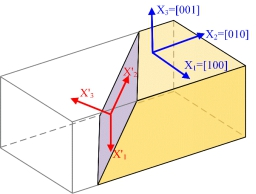
\includegraphics[width=0.6\textwidth]{figures/sample1.png}
  \caption{晶体坐标系和样品坐标系示意图}
  \label{fig:sample1}
\end{figure}

\begin{figure}[!htbp]
  \centering
  \subfloat[云图;]{
    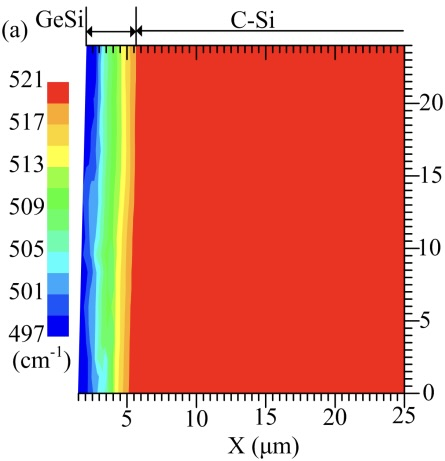
\includegraphics[height=0.38\textwidth]{figures/sample2L.jpeg}
  }
  \subfloat[沿深度方向分布曲线]{
    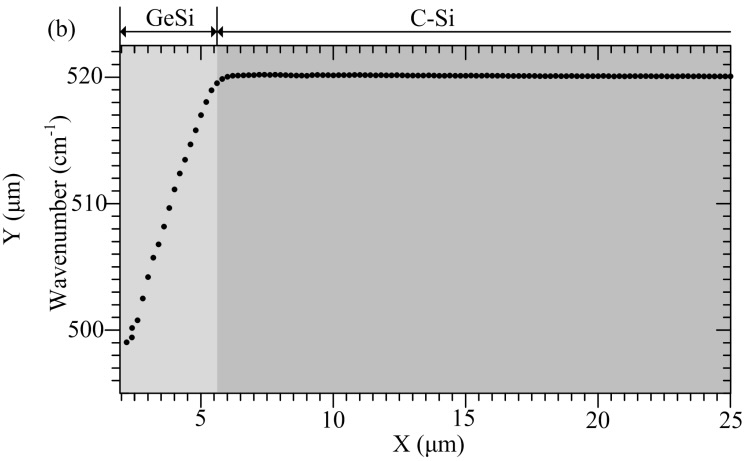
\includegraphics[height=0.38\textwidth]{figures/sample2R.jpeg}
  }
  \caption{应变硅横截面样品的拉曼类硅峰峰位}
  \label{fig:sample2}
\end{figure}


\subsection{表}

表中参数应标明量和单位的符号。表的编排建议采用国际通行的三线表。表与其前后的正文之间要有一行的间距;文中的表一律采用阿拉伯数字分章编号,如:表3-2。若表中有附注,采用英文小写字母顺序编号。表序及表题居中置于表的上方。如某个表需要转页接排,在随后的各页上应重复表序,后跟表题(可省略)和“(续)”,置于表格上方。续表均应重复表头。表序与表题之间空一个全角空格或两个半角空格。引用表应在表题右上角标出文献来源。表的附注应位于图或表的下方。

依照以上标准的三线表范例如下。

\begin{table}[!htbp]
  \centering
  \caption{典型微尺度力学实验方法的基本信息}
  \label{tab:tab1}
  \vspace{0.5em}
  \begin{tabular}{ccc}
    \toprule
    \textbf{实验方法} & \textbf{主要测量对象} & \textbf{空间分辨率}    \\
    \midrule
    原子力显微镜        & 表面力             & 0.1 nm {[}1{]}    \\
    透射电镜          & 晶格结构、位错         & 0.1 nm {[}2{]}    \\
    X射线衍射         & 应变              & 1 $\mu$m{[}3-5{]}     \\
    同步辐射          & 内部三维结构与变形       & 约100 nm{[}6, 7{]} \\
    显微拉曼          & 应变              & 250 nm {[}8{]}    \\ 
    \bottomrule
  \end{tabular}
\end{table}

\section{脚注}

在正文当中\footnote{脚注字号为五号,其余样式与正文相同。},如果有个别名词或情况需要解释时,可加注释说明。注释说明应采用文中编号加脚注的模式。脚注应采用阿拉伯数字上标,字体为Times New Roman,分页连续标号。脚注字号为五号,其余样式与正文相同。


\section{页眉和页脚}

页眉从正文开始到毕业设计(论文)结尾,一律设为“天津大学XX届本科生毕业设计(论文)”,采用五号字居中书写,其余样式与正文相同。

页脚从中文摘要开始,从 I 开始顺序编页码,为大写罗马数字格式。正文第一页开始,用阿拉伯数字重新从1开始顺序编页码,至学位论文结尾。页脚的字号为小五号,居中书写。

% \addcontentsline{toc}{chapter}{结\quad 论} %添加到目录中
% \chapter*{结\quad 论}

\chapter{实验与分析}

\section{任务书}
任务书内容应包括原始依据、参考文献、设计内容和要求,其中原始依据要填写明确,原始依据不得少于200字,包括设计(论文)的工作基础、研究条件、应用环境、工作目的;设计(研究)内容和要求不得少于200字,包括设计(研究)内容、主要指标与技术参数,并根据课题性质对学生提出具体要求。

\section{开题报告}
开题报告要求不少于2000字,内容包括:课题的来源及意义,国内外发展状况,本课题的研究目标、研究内容、研究方法、研究手段和进度安排,实验方案的可行性分析和已具备的实验条件以及主要参考文献等。

\section{评阅书}

\subsection{指导教师评阅书}

指导教师评阅书中的“评阅意见” 不能少于200字,主要包括对开题报告、设计或研究内容、外文资料和译文、工作量、工作态度、设计或论文质量、创新性、应用性、论文写作、文本规范、存在的不足和综合评价等方面的评阅意见,应体现对所评阅论文的具体意见,要有针对性。

\subsection{评阅教师评阅书}

评阅教师评阅书中的“评阅意见”不能少于200字,主要包括对选题、设计或研究内容、外文资料和译文、工作量、设计或论文质量、创新性、应用性、论文写作、文本规范、存在的不足和综合评价等方面的评阅意见,应体现对所评阅论文的具体意见,要有针对性。

\section{答辩记录书}

答辩记录书中的“综合评价”不能少于100字,主要包括设计或研究内容、工作量、设计或论文质量和答辩情况;“答辩记录”主要包含答辩委员提出的问题和学生回答情况等,答辩记录由答辩小组秘书填写。

\section{外文资料和中文译文}

外文资料要与所做课题紧密联系,严禁抄袭有中文译本的外文资料,外文资料的选取要注明出处。可用 A4纸复印,如果打印,标题应采用不编号章标题样式,内容应采用正文样式。中文译文的字数一般为5000 ~ 6000汉字。



%%%%%%%%%%  参考文献  %%%%%%%%%%
\newpage
\bibliographystyle{references/ref.buk}
\nocite{*}                                     % 若将此命令屏蔽掉,则未引用的文献不会出现在文后的参考文献中
\bibliography{references/reference}

% \include{appendix/paperInEnglish}              % 外文资料
% \include{appendix/paperInChinese}              % 中文译文

\addcontentsline{toc}{chapter}{\texorpdfstring{附\quad 录}{附录}}
%\setcounter{page}{1}       % 如果需要从该页开始从 1 开始编页,则取消该注释
\chapter*{\texorpdfstring{附\quad 录}{附录}}

附录的有无,根据毕业设计(论文)情况而定,内容一般包括正文内不便列出的冗长公式推导、辅助性数学工具、符号说明(含缩写)、计算程序及说明等。附录另起一页。附录依序用大写正体A、B、C、…编序号,如:附录A。附录中的图、表、公式、参考文献等另行编序号,与正文分开,也一律用阿拉伯数字编码,但在数码前冠以附录序码,如:图A01、表B-2、公式(B-3)、文献[A5]等。“附录”两字之间空一个全角空格或两个半角空格,采用不编号章标题样式;内容应采用正文样式。

\addcontentsline{toc}{chapter}{\texorpdfstring{致\quad 谢}{致谢}} % 添加到目录中
\chapter*{\texorpdfstring{致\quad 谢}{致谢}}

致谢应以简短的文字对课题研究与论文撰写过程中曾直接给予帮助的人员(例如指导教师)表示谢意。“致谢”两字之间空一个全角空格或两个半角空格,采用不编号章标题样式;内容应采用正文样式。
            % 致谢
\clearpage
\end{document}                                 % 结束全文
